\documentclass[a4paper,12pt]{article}
%%%%%%%%%%%%%%%%%%%%%%%%%%%%%%%%%%%%%%%%%%%%%%%%%%%%%%%%%%%%%%%%%%%%%%%%%%%%%%%%%%%%%%%%%%%%%%%%%%%%%%%%%%%%%%%%%%%%%%%%%%%%%%%%%%%%%%%%%%%%%%%%%%%%%%%%%%%%%%%%%%%%%%%%%%%%%%%%%%%%%%%%%%%%%%%%%%%%%%%%%%%%%%%%%%%%%%%%%%%%%%%%%%%%%%%%%%%%%%%%%%%%%%%%%%%%
\usepackage{eurosym}
\usepackage{vmargin}
\usepackage{amsmath}
\usepackage{graphics}
\usepackage{epsfig}
\usepackage{enumerate}
\usepackage{multicol}
\usepackage{subfigure}
\usepackage{fancyhdr}
\usepackage{listings}
\usepackage{framed}
\usepackage{graphicx}
\usepackage{amsmath}
\usepackage{chngpage}
%\usepackage{bigints}

\usepackage{vmargin}
% left top textwidth textheight headheight
% headsep footheight footskip
\setmargins{2.0cm}{2.5cm}{16 cm}{22cm}{0.5cm}{0cm}{1cm}{1cm}
\renewcommand{\baselinestretch}{1.3}

\setcounter{MaxMatrixCols}{10}
\begin{document}
	
	%%%%%%%%%%%%%%%%%%%%%%%%%%%%%%%%%%%%%%%%%%%%%%%%%%%%%%%%%%%%%%%%%%%%%%%%%%%%%%%%%%%%%%%%%%%%%%%%%%%%%%%%%%%%%%%%%%%%%
	\begin{table}[ht!]
		
		\centering
		
		\begin{tabular}{|p{15cm}|}
			
			\hline  
			
			%%-- 8. (a) 
			\large
			\noindent Discuss the advantages and disadvantages of using non-parametric rather than parametric methods in statistical analyses.
			\\ \hline
			
		\end{tabular}
		
	\end{table}
	\large
\noindent	Parametric methods require a distribution (often the normal) to be specified as a model for
	the observations. 
	\begin{itemize}
		\item If this is not correct, inferences can be seriously affected.\item Non-parametric methods
		rely on such things as rank ordering of data, and require no distributional assumptions. 
		\item They
		allow more general types of analysis, not based on means and variances (parameters) but are less
		powerful than parametric methods when they are available for the corresponding problem.
	\end{itemize}
	
	%%%%%%%%%%%%%%%%%%%%%%%%%%%%%%%%%%%%%%%%%%%%%%%%%%%%%%%%%%%%%%%%%%%%%%%%%%%%%%%%%%%%%%%%%%%%%%%%%%%%%%%%%%%%%%%%%%%%%
	\newpage
	
	\begin{table}[ht!]
		
		\centering
		
		\begin{tabular}{|p{15cm}|}
			
			\hline  
			\large
			\noindent The weights of fish in two populations were compared by analysing the differences in the weights of a random sample of fish from each population matched by length.  The weight differences in grams for 10 pairs of fish was as follows:
			\[ \{12,\; -13,\;-125,\;-120,\;-73,\;2,\;3,\;-147,\;-12,\;-4 \}\]
			Explain why a parametric test would be unsuitable for comparing the weights of the fish from these two populations.
			Analyse these data using a test which:
			\begin{enumerate}[(i)]
				\item ignores the magnitudes of the differences,
				\item uses both the signs and magnitudes of the differences.
			\end{enumerate}
			Comment on the comparison of your results.
			
			\\ \hline
			
		\end{tabular}
		
	\end{table}
	
	%%%%%%%%%%%%%%%%%%%%%%%%%%%%%%%%%%%%%%%%%%%%%%%%%%%%%%%%%%%%%%%%%%%%%%%%%%%%%%%%%%%%%%%%%%%%%%%%%%%%%%%%%%%%%%%%%%%%%
	
	
	\large
	\begin{itemize}
		\item 
		These data are very skewed. %, even after differences have been taken. 
		\item Even if a logarithmic transformation
		is taken, the resulting data cannot be taken as anywhere near symmetrical.
		\item A sign test uses only +/-, and there are 3 ``+``s, 7 ``-``s in 10 pairs. If the populations are the
		same, $H_0$ says that the proportion of ``+`` signs is $ \frac{1}{2}$ , so the number of ``+``s is Binomial(10,1/2).
		
		%%%%%%%%%%%%%%%%%%%%%%%%%%%%%%%%%%%%%%%%%%%%%%%%%%%
		\newpage
		\begin{framed}
			\begin{verbatim}
			> dbinom(0,10,0.5)
			[1] 0.0009765625
			>
			> dbinom(1,10,0.5)
			[1] 0.009765625
			>
			> dbinom(2,10,0.5)
			[1] 0.04394531
			>
			> dbinom(3,10,0.5)
			[1] 0.1171875
			>
			> pbinom(3,10,0.5)
			[1] 0.171875
			\end{verbatim}
		\end{framed}
		\noindent \textbf{Calculate P-Value}\\
		\begin{eqnarray*}
			P(\leq \;3 ``+``s) &=& P(0) +P(1) +P(2) +P(3) \\
			&=& \frac{1}{2^{10}} (1 + 10 + 45 + 120) \\
			&=& 0.172.\\
		\end{eqnarray*}
		This p-value is $>0.05$, so does not provide evidence of any difference.
		
		\newpage
		\item Wilcoxon’s signed ranks test uses both signs and magnitudes.
		\begin{description}
			\item[ $H_0$] “populations are the same”, 
			\item[ $H_1$] “populations are different”. 
		\end{description}
		\subsection*{Ranked absolute values}
		
		\begin{center}
			\begin{tabular}{|c|c|c|c|c|c|c|c|c|c|c|c|} \hline
				$|\mbox{diff}|$ & 2 & 3 & 4 & 12 & 12 & 13 & 73 & 120 & 125 & 147\\ \hline
				rank & 1 & 2 & 3 & 4 $\frac{1}{2}$ & 4 $\frac{1}{2}$ &  6 & 7 & 8 & 9 & 10 \\ \hline
				sign & \;+\;& \;+\;&  \;- \;& \;+\;& \;-\;& \;-\;&\; -\;& \;-\;& \;-\;& \;-\;\\ \hline
			\end{tabular}
		\end{center}
		\begin{itemize}
			\item The sum of the positive ranks is $7\frac{1}{2}$ and is below the (2-sided) critical table value 8 for $n=10$,
			and so the Null Hypothesis is rejected.
			\item  Using this test, there is evidence of different location of population
			values.
			\item By using the values, more information is available, since the $+$ signs are attached to values
			that are numerically quite small. 
			\item The Wilcoxon test thus gains greater power to discriminate between
			the two sets of data that produced the differences given.
		\end{itemize}
		
	\end{itemize}
	
	\newpage
	
\begin{figure}
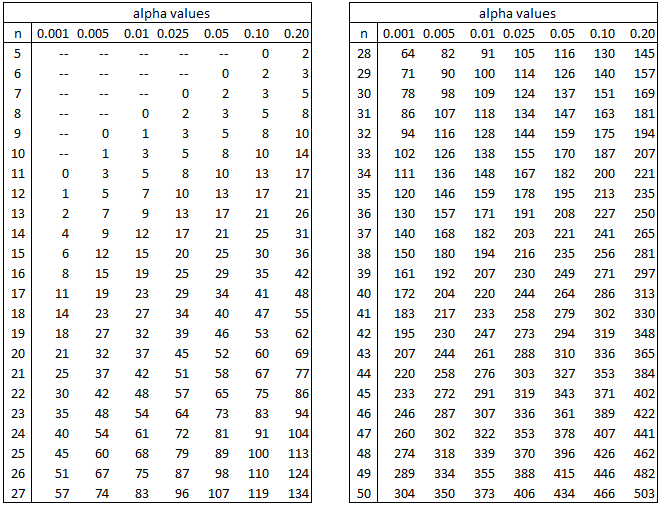
\includegraphics{images/signed-ranks-table}
\caption{}
\label{fig:signed-ranks-table}
\end{figure}
\end{document}
